\chapter{T-이중성, D-브레인과 게이지 이론}

\lectureoverview{T-이중성은 반지름이 (R)인 원 위의 닫힌 끈과 \(\alpha'/R\)인 원 위의 닫힌 끈 사이의 정확한 동등성으로 시작한다. 운동량과 감김수의 역할이 서로 바뀌고, 세계면 미분 \(\partial_\tau Y\)와 \(\partial_\sigma Y\), 그리고 \(G_{\mu 5}\)와 \(B_{\mu 5}\)에서 유래하는 시공간 벡터장도 서로 바뀐다. 같은 변환을 열린 끈에 적용하면 노이만 끝점 조건이 디리클레 조건으로 바뀐다. 그러면 끝점은 동역학적 D-브레인 위에 놓여야 한다. 하나의 브레인에 붙들린 열린 끈은 저에너지에서 아벨 게이지 이론을 이루고, 브레인 더미를 잇는 끈은 양 끝점의 꼬리표를 지녀 비아벨 게이지 이론을 이룬다. D3-브레인에 끝나는 D-끈은 그에 대응하는 자기 홀극을 제공한다.}

\section{왜 T-이중성으로 돌아가는가?}

우리는 이미 T-이중성을 살펴보았지만, 여기에는 다시 다룰 이유가 있다. T-이중성은 끈 이론에 섭동적 끈보다 훨씬 많은 것이 들어 있음을 보여 준 단서 가운데 하나였다. 열린 끈에 미치는 결과를 이해하면서 D-브레인이 등장했고, 이어서 D-브레인은 양자장 이론을 구성하고 연구하는 방법이 되었다. 따라서 이 강의의 목적은 작은 원이 큰 원과 동등하다는 표어를 되풀이하는 데 그치지 않는다. 그 표어가 이론에 새로운 물리적 대상을 어떻게 불러들이는지 알 수 있도록 논증을 차근차근 다시 세워 보겠다.

가장 단순한 설정은 토러스 콤팩트화다. 1차원 토러스는 원이다. 2차원 토러스는 마주 보는 변을 서로 식별한 평행사변형으로 나타낼 수 있고, 3차원 토러스는 마주 보는 면을 서로 식별한 평행육면체로 나타낼 수 있다. 같은 구성은 더 높은 차원에서도 이어진다. 콤팩트한 공간 좌표 하나만 남겨 \(Y\)라 하고, 비콤팩트 좌표 하나를 대표로 두어 \(X\)라 하겠다. 시간도 있지만 칠판 그림에는 표시하지 않는다.

다음 표준 관례를 택하자.
\begin{equation}
  Y\sim Y+2\pi R,
  \label{eq:l10-circle-identification}
\end{equation}
이에 따라 \(R\)는 반지름이고 \(2\pi R\)는 원주다. 강의에서는 콤팩트 방향의 크기를 흔히 간단히 \(r\)라 하고 \(2\pi\)와 \(\alpha'\)의 인자를 생략한다. 유도 과정에서는 표준 인자를 유지하고, 유용한 경우에는 강의에서 사용한 단위계의 표현도 보이겠다.

논의의 전반부에서는 닫힌 유향 끈을 다룬다. 방향은 끈을 따라 그린 본질적인 화살표다. 어디서나 모든 화살표를 뒤집어도 실험 결과는 달라지지 않는다. 중요한 것은 두 끈 사이의 상대적 방향이다. 끈이 갈라지거나 합쳐질 때 화살표는 연속적으로 이어져야 한다. 이것은 부호를 지닌 보존량이 나타나리라는 첫 번째 단서다.

\begin{figure}[H]
  \centering
  \includegraphics[width=0.72\textwidth]{lecture_10_figure_01.png}
  \caption{칠판에 상대적 방향을 표시한 두 닫힌 끈. 분할과 결합 과정에서도 방향은 연속적이어야 한다.}
  \lectureframe{00:05:40}
  \label{fig:l10-oriented-closed-strings}
\end{figure}

\begin{classroomqa}
\audiencequestion{세계면 좌표가 \(\sigma=0\)에서 \(2\pi\)까지 변한다면, 끈은 이미 콤팩트 방향을 한 바퀴 돈 것인가? \lecturetimestamp{00:08:42}}
\lecturerresponse{아니다. 좌표 \(\sigma\)는 끈을 따라 있는 점들을 표시할 뿐, 콤팩트 공간에서의 위치를 표시하지 않는다. 감겼든 풀렸든 모든 닫힌 끈에는 주기 매개변수 \(\sigma\)가 있다. 고무줄의 비유가 도움이 된다. 고무줄을 아무것에도 감지 않았더라도 둘레를 따라 있는 분자에 번호를 매길 수 있다. 감김은 매개변수 \(\sigma\) 자체가 아니라 사상 \(Y(\tau,\sigma)\)의 성질이다.}
\end{classroomqa}

\begin{classroomqa}
\audiencequestion{콤팩트 방향의 크기도 큰 좌표 \(X\)의 모든 값에서 같아야 하나요? \lecturetimestamp{00:10:00}}
\lecturerresponse{일반적인 동역학적 콤팩트화에서는 그렇지 않다. 가장 단순한 배경인 고정된 원에서 시작하겠다. 나중에는 성분 \(G_{55}\)가 다섯 번째 방향의 국소적 크기를 나타내는 스칼라장이 되어, 그 크기가 보통 시공간에 걸쳐 달라질 수 있다.}
\end{classroomqa}

\section{끈들이 다시 연결되어도 감김수는 보존된다}

감기지 않은 끈은 감기지 않은 채 콤팩트 방향을 따라 움직일 수 있다. 감긴 끈은 다르다. \(\sigma\)가 닫힌 끈을 따라 한 바퀴 돌 때 매장 \(Y(\tau,\sigma)\)은 콤팩트 원의 주기를 하나 이상 진행한다. 끈에는 방향이 있으므로 진행 방향에는 부호가 붙는다. 끈은 양의 방향으로 감길 수도 있고 음의 방향으로 감길 수도 있다.

결합 그림을 보면 보존 법칙이 가장 분명하게 드러난다. 감김수 \(+1\)인 끈 하나와 감김수 \(-1\)인 다른 끈 하나를 생각하자. 두 끈의 방향이 맞는 구간은 다시 연결될 수 있다. 그렇게 얻은 배치의 총 감김수는 0이며, 이를 감기지 않은 끈으로 변형할 수 있다. 칠판 그림은 방향이 반대인 끈들이 다시 연결되는 바로 그 과정을 보여 준다.

\begin{figure}[H]
  \centering
  \includegraphics[width=0.72\textwidth]{lecture_10_figure_02.png}
  \medskip

  \begin{tikzpicture}[x=1cm,y=1cm,>=Latex]
    \draw[thick] (-4.0,0.3) circle (0.65);
    \draw[->,thick] (-4.55,0.58) arc (150:-145:0.65);
    \node at (-4.0,-0.65) {$w=+1$};
    \draw[thick] (-2.0,0.3) circle (0.65);
    \draw[<-,thick] (-2.55,0.58) arc (150:-145:0.65);
    \node at (-2.0,-0.65) {$w=-1$};
    \node at (-3.0,0.3) {$+$};
    \draw[->,thick] (-1.0,0.3) -- (0.3,0.3);
    \draw[thick] (1.4,0.3) ellipse (0.95 and 0.55);
    \node at (1.4,-0.65) {$w_{\rm total}=0$};
  \end{tikzpicture}
  \caption{반대 방향의 감김이 다시 연결되어 총 감김수가 0인 배치가 된다. 아래 그림은 칠판의 과정을 깔끔하게 다시 그린 것이며, 별도의 동역학적 과정이 아니다.}
  \lectureframe{00:13:20}
  \label{fig:l10-opposite-winding}
\end{figure}

이번에는 방향이 같은 끈 두 개로 실험을 반복해 보자. 이 끈들은 합쳐질 수 있지만 감김을 풀 수는 없다. 결과로 생긴 끈의 감김수는 들어온 각 끈의 감김수의 두 배다. 연결된 끈의 개수는 바뀌었지만 총 감김수는 바뀌지 않았다.

\begin{figure}[H]
  \centering
  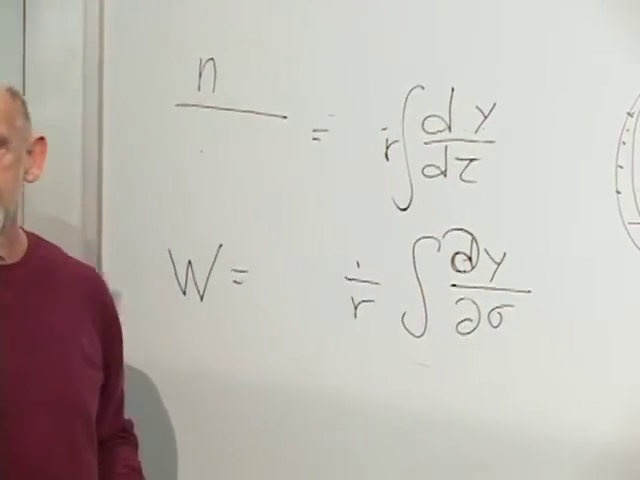
\includegraphics[width=0.72\textwidth]{lecture_10_figure_03.png}
  \medskip

  \begin{tikzpicture}[x=1cm,y=1cm,>=Latex]
    \draw[thick] (-4.0,0.3) circle (0.65);
    \draw[->,thick] (-4.55,0.58) arc (150:-145:0.65);
    \node at (-4.0,-0.65) {$w=+1$};
    \draw[thick] (-2.0,0.3) circle (0.65);
    \draw[->,thick] (-2.55,0.58) arc (150:-145:0.65);
    \node at (-2.0,-0.65) {$w=+1$};
    \node at (-3.0,0.3) {$+$};
    \draw[->,thick] (-1.0,0.3) -- (0.3,0.3);
    \draw[thick] (1.45,0.3) circle (0.78);
    \draw[thick] (1.45,0.3) circle (0.52);
    \draw[->,thick] (0.81,0.74) arc (145:-145:0.78);
    \node at (1.45,-0.78) {$w=+2$};
  \end{tikzpicture}
  \caption{같은 부호의 감김은 다시 연결되어 감김수가 두 배인 끈이 될 수 있다. 연결 상태는 달라져도 총 감김수 2는 유지된다.}
  \lectureframe{00:16:40}
  \label{fig:l10-same-winding}
\end{figure}

이 구분은 허용되는 모든 과정에서 유지된다. 총 감김수 100은 100번 감긴 끈 하나, 각각 50번 감긴 끈 두 개, 또는 한 번씩 감긴 끈 100개가 지닐 수 있다. 끈은 이 여러 형태 사이에서 갈라지고 합쳐질 수 있지만, 부호를 포함한 합은 계속 100이다. 이를 \(w\in\mathbb Z\)로 나타낸다.

\section{운동량 모드와 감김 모드}

보존만으로는 아직 쌍대성이 성립하는 것은 아니다. 다음으로 에너지를 비교해 보자. 콤팩트 원을 따라 움직이는 상태는 양자화된 운동량을 갖는다
\begin{equation}
  p_Y=\frac{n}{R},
  \qquad n\in\mathbb Z.
  \label{eq:l10-compact-momentum}
\end{equation}
다른 질량 기여를 무시할 수 있는 상태에서는 콤팩트 방향 운동이 \(E_{\rm mom}=|n|/R\)에 기여한다. \(n\)의 양수와 음수는 서로 반대 방향의 운동을 뜻하지만, 에너지는 양수다.

\begin{figure}[H]
  \centering
  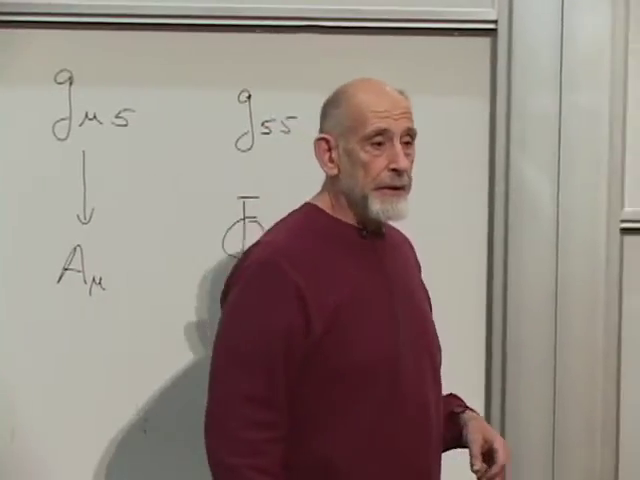
\includegraphics[width=0.72\textwidth]{lecture_10_figure_04.png}
  \caption{칠판에 적힌 콤팩트 운동량의 양자수. 강의에서는 운동량을 콤팩트 방향 속도의 적분으로 개략적으로 쓴다.}
  \lectureframe{00:21:30}
  \label{fig:l10-compact-momentum-board}
\end{figure}

\(|w|\)번 감긴 끈의 길이는 \(2\pi |w|R\)다. 기본 끈 장력을
\begin{equation}
  T_{\rm F}=\frac{1}{2\pi\alpha'},
\end{equation}
이라 하면, 감김 에너지는 다음과 같다.
\begin{equation}
  E_{\rm wind}=T_{\rm F}(2\pi |w|R)
  =\frac{|w|R}{\alpha'}.
  \label{eq:l10-winding-energy}
\end{equation}
강의에서 사용하는 단위계 \(\alpha'=1\)에서는 간단히 \(E_{\rm wind}=|w|R\)다.

반지름이 변할 때 두 에너지 탑은 서로 반대로 변한다. \(R\gg
\sqrt{\alpha'}\)이면 운동량 준위의 간격은 좁고 감김 준위의 간격은 넓다. \(R\ll\sqrt{\alpha'}\)이면 운동량 준위의 간격은 넓고 감김 준위의 간격은 좁다.

\begin{figure}[H]
  \centering
  \begin{minipage}[t]{0.48\textwidth}
    \centering
    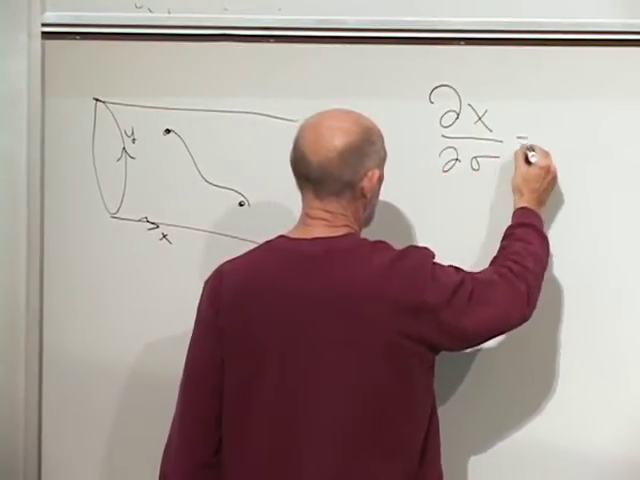
\includegraphics[width=\linewidth]{lecture_10_figure_05.png}
    \par\smallskip
    \textit{큰 콤팩트 반지름.}
  \end{minipage}\hfill
  \begin{minipage}[t]{0.48\textwidth}
    \centering
    \includegraphics[width=\linewidth]{lecture_10_figure_06.png}
    \par\smallskip
    \textit{작은 콤팩트 반지름.}
  \end{minipage}
  \caption{칠판에 나타난 두 스펙트럼을 비교한 그림. 반지름을 역수로 바꾸면 성긴 탑과 조밀한 탑의 역할이 서로 바뀐다.}
  \lectureframe{00:25:30--00:26:00}
  \label{fig:l10-dual-spectra-board}
\end{figure}

개략적인 관계는 다음과 같다.
\begin{figure}[H]
  \centering
  \begin{adjustbox}{max width=\linewidth}
  \begin{tikzpicture}[x=1cm,y=0.74cm,>=Latex]
    \node[font=\bfseries] at (-3.6,6.2) {$R\gg\sqrt{\alpha'}$};
    \draw[->] (-5.1,0) -- (-5.1,5.5) node[above] {$E$};
    \foreach \y in {0.4,1.0,1.6,2.2,2.8,3.4,4.0,4.6}
      \draw (-5.35,\y)--(-4.85,\y);
    \node[align=center] at (-4.25,5.15) {momentum\\dense};
    \draw[->] (-2.2,0) -- (-2.2,5.5) node[above] {$E$};
    \foreach \y in {0.4,2.4,4.4}
      \draw (-2.45,\y)--(-1.95,\y);
    \node[align=center] at (-1.35,5.15) {winding\\sparse};

    \node[font=\bfseries] at (3.6,6.2) {$R\ll\sqrt{\alpha'}$};
    \draw[->] (2.2,0) -- (2.2,5.5) node[above] {$E$};
    \foreach \y in {0.4,2.4,4.4}
      \draw (1.95,\y)--(2.45,\y);
    \node[align=center] at (3.05,5.15) {momentum\\sparse};
    \draw[->] (5.1,0) -- (5.1,5.5) node[above] {$E$};
    \foreach \y in {0.4,1.0,1.6,2.2,2.8,3.4,4.0,4.6}
      \draw (4.85,\y)--(5.35,\y);
    \node[align=center] at (5.95,5.15) {winding\\dense};
  \end{tikzpicture}
  \end{adjustbox}
  \caption{준위 간격 논증을 다시 그린 그림. 운동량과 감김을 서로 바꾸고 \(R\leftrightarrow\alpha'/R\)도 함께 바꾸어도 끈의 전체 스펙트럼은 변하지 않는다.}
  \label{fig:l10-dual-spectra-redraw}
\end{figure}

관찰자에게 이 스펙트럼 가운데 하나를 보여 주되 어떻게 얻었는지는 알려 주지 않았다고 하자. 간격이 좁은 탑은 큰 원 위의 운동량 탑일까, 작은 원 위의 감김 탑일까? 스펙트럼만으로는 알 수 없다. 끈 이론은 더 강한 주장을 한다. 산란 진폭으로도 둘을 구별할 수 없다는 것이다. 두 기술은 다음 변환 아래에서 정확히 동등하다.
\begin{equation}
  n\longleftrightarrow w,
  \qquad
  R\longleftrightarrow \widetilde R=\frac{\alpha'}{R}.
  \label{eq:l10-radius-duality}
\end{equation}
자기 자신으로 대응되는 고정점은
\begin{equation}
  R=\sqrt{\alpha'},
  \label{eq:l10-self-dual-radius}
\end{equation}
이며, 강의 단위계에서는 \(R=1\)다. 이 반지름에서는 추가 상태가 질량 없는 상태가 될 수 있고 게이지 대칭이 확장된다.

\begin{classroomqa}
\audiencequestion{감김은 스펙트럼을 다시 쓰기 위한 수학적 편의에 불과한가요? \lecturetimestamp{00:27:33}}
\lecturerresponse{아니다. 감김은 닫힌 끈 힐베르트 공간의 실제 부문을 나타내며, 이 부문들은 상호작용에 참여한다. ``이중성''이란 운동량 기술과 감김 기술이 동일한 물리의 서로 다른 좌표라는 뜻이다. 한 부문이 다른 부문을 대신해 선택적으로 쓰는 기억법이라는 뜻이 아니다.}
\end{classroomqa}

\begin{classroomqa}
\audiencequestion{자기 자신으로 대응되는 반지름이 있나요?
\lecturetimestamp{00:27:58}}
\lecturerresponse{있다. 자기이중 값은 \(R=\sqrt{\alpha'}\)이며, 칠판에서 사용한 단위계로는 \(R=1\)다. 이곳에서 두 탑이 만나고 스펙트럼의 대칭성이 확장된다.}
\end{classroomqa}

\section{이중성의 세계면 표현}

스펙트럼을 이용한 논증은 이중성을 시사하지만, 세계면을 보면 두 양의 교환을 더 정확히 나타낼 수 있다. 등각 게이지에서 \(Y\)에 켤레인 운동량은 \(\partial_\tau Y\)에 비례한다. 따라서 전체 콤팩트 운동량은 다음과 같다.
\begin{equation}
  P_Y=\frac{1}{2\pi\alpha'}
      \int_0^{2\pi}d\sigma\,\partial_\tau Y.
  \label{eq:l10-worldsheet-momentum}
\end{equation}
감김수는 다음과 같다.
\begin{equation}
  w=\frac{1}{2\pi R}
      \int_0^{2\pi}d\sigma\,\partial_\sigma Y
   =\frac{Y(2\pi)-Y(0)}{2\pi R}.
  \label{eq:l10-worldsheet-winding}
\end{equation}

\begin{classroomqa}
\audiencequestion{닫힌 끈을 따라 미분을 적분했는데도 왜 사라지지 않는가? \lecturetimestamp{00:32:33}}
\lecturerresponse{\(Y\)는 주기적인 표적 공간 좌표이지 \(\sigma\)-원 위에서 단일값을 갖는 실수 함수가 아니기 때문이다. 세계면의 점 \(\sigma=2\pi\)는 \(\sigma=0\)와 같은 점이지만, 매장을 덮개 직선 위로 올리면 \(2\pi wR\)만큼 변한다. \(\partial_\sigma Y\)의 적분은 그 이동량을 측정한다.}
\end{classroomqa}

\begin{figure}[H]
  \centering
  \includegraphics[width=0.76\textwidth]{lecture_10_figure_07.png}
  \caption{칠판에서 두 식을 모두 완성한 뒤의 운동량 적분과 감김 적분. 강의의 정규화에서는 공통 인자 \(2\pi\)와 \(\alpha'\)를 생략한다.}
  \lectureframe{00:33:25}
  \label{fig:l10-momentum-winding-integrals}
\end{figure}

한 번 감긴 끈의 경우,
\begin{equation}
  Y(\tau,\sigma+2\pi)=Y(\tau,\sigma)+2\pi R.
\end{equation}
감김수가 \(w\)이면 우변의 변위는 \(2\pi wR\)이다. 그러면 식 \eqref{eq:l10-worldsheet-winding}는 감김수를 정확히 센다. 이것이 칠판의 약식 표기 \(w\sim R^{-1}\int
d\sigma\,\partial_\sigma Y\)를 엄밀히 나타낸 것이다.

따라서 T-이중성의 세계면 표현은 다음과 같다.
\begin{equation}
  \partial_\tau Y\longleftrightarrow
  \partial_\sigma \widetilde Y,
  \qquad
  \partial_\sigma Y\longleftrightarrow
  \partial_\tau \widetilde Y,
  \label{eq:l10-derivative-duality}
\end{equation}
여기서는 \(Y\)의 운동량이 이중 좌표 \(\widetilde Y\)의 감김으로 바뀌며, 그 반대도 성립한다.

\begin{classroomqa}
\audiencequestion{그렇다면 세계면 좌표 \(\tau\)와 \(\sigma\) 자체가 서로 대응하거나 뒤바뀌나요?
\lecturetimestamp{00:34:39}}
\lecturerresponse{아니다. T-이중성은 해를 서로 대응시키고 콤팩트 표적 공간 좌표의 특정 미분을 교환한다. 세계면의 시간 좌표와 공간 좌표를 동일시하지 않는다.}
\end{classroomqa}

\section{감김 상태를 피할 수 없는 이유}

감기지 않은 상태가 있는데도 끈이 왜 감긴 상태로 나타나겠느냐고 물을 수 있다. 끈은 선호에 따라 상태를 선택하지 않는다. 충돌에서 공급된 에너지는 끈을 늘린다. 충분히 높은 에너지를 지닌 크게 변형된 끈은 서로 반대 방향으로 감긴 두 끈으로 다시 연결될 수 있다. 두 끈의 총 감김수는 여전히 0이지만, 분할 뒤에는 서로 멀어질 수 있다. 한 끈을 멀리 보내면 관찰자에게는 감긴 끈 하나만 고립되어 있는 듯 보일 수 있다.

\begin{figure}[H]
  \centering
  \includegraphics[width=0.76\textwidth]{lecture_10_figure_08.png}
  \caption{다시 연결된 뒤 서로 반대 방향으로 감긴 끈들이 분리될 수 있는, 크게 늘어난 총 감김수 0의 배치.}
  \lectureframe{00:36:15}
  \label{fig:l10-winding-pair-production}
\end{figure}

에너지 문턱은 감김 에너지로 정해진다. 큰 원에서는 콤팩트 방향을 충분히 감쌀 만큼 끈을 늘리려면 높은 충돌 에너지가 필요하다. 하지만 문턱을 넘으면 감김--반감김 쌍생성을 금지할 수 없다. 이는 광자 충돌로 전자--양전자가 생성되는 것과 비슷하다. 총 전하는 여전히 0이지만, 하전 입자들이 실제로 생겨 서로 떨어질 수 있다. 감김수 보존도 같은 방식으로 작동한다.

이 비유는 말뿐인 유사성이 아니다. 콤팩트 운동량과 감김은 서로 구별되는 두 전하 양자수처럼 작용한다. 이에 대응하는 저차원 기술에서 같은 부호끼리는 밀어내고 반대 부호끼리는 끌어당긴다. 그러므로 이 힘을 매개하는 두 벡터장을 찾아야 한다.

\section{5차원 중력에서 얻는 운동량 전하}

5차원 중력에서 시작하자. 대문자 첨자 \(M,N\)는 네 개의 보통 시공간 방향과 콤팩트한 다섯 번째 방향을 모두 가리킨다. 계량은 다음과 같이 분해된다.
\begin{equation}
  G_{MN}\quad\longrightarrow\quad
  \bigl\{G_{\mu\nu},\,G_{\mu5},\,G_{55}\bigr\}.
  \label{eq:l10-metric-decomposition}
\end{equation}
대칭성분 \(G_{5\mu}\)에는 \(G_{\mu5}\)에 이미 포함된 정보 외에 새로운 정보가 없다.

\begin{figure}[H]
  \centering
  \includegraphics[width=0.74\textwidth]{lecture_10_figure_09.png}
  \caption{서로 독립적인 5차원 계량 성분의 묶음: \(G_{\mu\nu}\), \(G_{\mu5}\), \(G_{55}\).}
  \lectureframe{00:44:05}
  \label{fig:l10-metric-components}
\end{figure}

4차원 관점에서 보면,
\begin{align}
  G_{\mu\nu} &\quad\hbox{is a spacetime metric},\\
  G_{\mu5} &\equiv A_\mu\quad\hbox{is a vector field},\\
  G_{55} &\equiv e^{2\varphi}\quad\hbox{is a scalar modulus}.
  \label{eq:l10-four-dimensional-fields}
\end{align}
스칼라 \(\varphi\)는 콤팩트 방향의 크기를 나타낸다. 이 값은 보통 시공간에 걸쳐 매끄럽게 변할 수 있으므로, \(\varphi\)의 파동은 다섯 번째 차원의 반지름이 요동하는 파동이다.

\begin{figure}[H]
  \centering
  \includegraphics[width=0.74\textwidth]{lecture_10_figure_10.png}
  \caption{칠판에서는 \(G_{\mu5}\)를 벡터 \(A_\mu\)와, \(G_{55}\)을 스칼라 \(\Phi\)와 대응시킨다.}
  \lectureframe{00:47:40}
  \label{fig:l10-vector-and-radius-modulus}
\end{figure}

혼합 중력 성분의 원천은 혼합 운동량 흐름이다. 특히 다섯 번째 방향을 따른 운동량은 \(G_{\mu5}\)의 원천이 된다. 따라서 4차원 관찰자는 정수 \(n\)를 \(A_\mu\)에 결합하는 전하로 해석한다. 이것이 칼루차--클라인 메커니즘이다. 고차원 기하에서 운동량이던 것이 저차원 장 이론에서는 전하가 된다.

\editorialnote{\(G_{55}\)에서 나온 스칼라를 강의에서는 느슨하게 ``딜라톤''이라고 부른다. 이 축약에서 이 스칼라는 구체적으로 반지름 모듈러스다. 끈 결합을 조절하는 10차원 끈 딜라톤은 별개의 장이지만, 기준계와 이중성을 바꾸면 저차원 스칼라의 조합들이 서로 섞일 수 있다.}

\begin{classroomqa}
\audiencequestion{스칼라 \(\varphi\)는 운동량 정수 \(n\)에 비례하나요? \lecturetimestamp{00:48:43}}
\lecturerresponse{아니다. 정수 \(n\)는 양자화된 상태를 표시하고 전하로 작용한다. 스칼라 \(\varphi(x)\)는 콤팩트화의 국소적 크기를 정하는 연속장이다. 위치에 따라 달라질 수 있으며, 그 자체가 정수인 것은 아니다.}
\end{classroomqa}

\section{두 번째 벡터장과 감김 전하}

감김도 전하와 비슷한 양이지만, 같은 벡터장에 같은 방식으로 결합할 수는 없다. 두 번째 벡터장을 보려면 최초의 닫힌 끈 들뜸으로 돌아가자. 닫힌 끈에는 왼쪽 진행 진동 모드와 오른쪽 진행 진동 모드가 있다. 물리적 상태는 레벨 정합 조건을 만족해야 한다. 즉 왼쪽 진행과 오른쪽 진행의 총 들뜸 준위가 서로 같아야 한다.

보손 이론에서 들뜸이 없는 상태는 타키온이다. 왼쪽 진행 또는 오른쪽 진행 진동자 하나만 들뜨면 레벨 정합을 어긴다. 따라서 처음으로 허용되는 질량 없는 상태에는 각 종류의 진동자가 하나씩 포함된다.
\begin{equation}
  \alpha_{-1}^{I}\widetilde\alpha_{-1}^{J}\ket{0;k}.
  \label{eq:l10-first-massless-state}
\end{equation}
첨자 \(I,J\)는 콤팩트 방향을 포함하는 횡방향 공간 성분을 가리킨다. 한 첨자는 보통 방향을, 다른 첨자는 \(5\)를 가리키면 벡터형 진동자 상태 두 개가 생긴다.
\begin{equation}
  \alpha_{-1}^{\mu}\widetilde\alpha_{-1}^{5}\ket{0;k},
  \qquad
  \alpha_{-1}^{5}\widetilde\alpha_{-1}^{\mu}\ket{0;k}.
  \label{eq:l10-two-vector-states}
\end{equation}

\begin{figure}[H]
  \centering
  \includegraphics[width=0.76\textwidth]{lecture_10_figure_11.png}
  \caption{왼쪽--오른쪽 진동자의 두 배열 순서. 편광 가운데 하나가 콤팩트 방향을 가리키면 4차원 벡터 상태가 된다.}
  \lectureframe{00:58:20}
  \label{fig:l10-two-vector-states-board}
\end{figure}

대칭 조합과 반대칭 조합은 서로 다른 시공간 장에 속한다.
\begin{align}
  \alpha_{-1}^{(\mu}\widetilde\alpha_{-1}^{5)}\ket{0;k}
    &\longleftrightarrow G_{\mu5},\\
  \alpha_{-1}^{[\mu}\widetilde\alpha_{-1}^{5]}\ket{0;k}
    &\longleftrightarrow B_{\mu5}.
  \label{eq:l10-g-and-b-vectors}
\end{align}
첫 번째는 콤팩트 운동량이 원천인 칼루차--클라인 벡터다. 두 번째는 반대칭 칼브--라몽 장에서 유래하며 끈 감김이 원천이다. 따라서 축약된 이론에는 각 전하 부문에 하나씩, 광자와 비슷한 장 두 개가 들어 있다.

두 진동자 첨자가 모두 콤팩트 방향을 가리키면 그 상태는 콤팩트화 모듈러스에 대응하는 스칼라다. 두 첨자가 모두 보통 횡방향을 가리키면 대칭 무대각합 성분은 중력자이고, 반대칭 성분은 \(B_{\mu\nu}\)이며, 대각합 성분은 스칼라 부문에 기여한다.

\begin{classroomqa}
\audiencequestion{이 상태 가운데 어느 것이 단일항이고 어느 것이 삼중항인가요? \lecturetimestamp{01:00:21}}
\lecturerresponse{여기서는 그 분류가 유용하지 않다. 혼합 상태 두 개 모두 4차원 벡터로 변환된다. 이들의 합과 차는 계량의 대칭 편광과 반대칭 \(B\)장 편광을 분리한다. 콤팩트 첨자 두 개를 지닌 상태는 4차원 스칼라다.}
\end{classroomqa}

휴식 전에 도달한 전체 대응 관계는 다음과 같다.
\begin{equation}
  \boxed{
  \begin{gathered}
    n\leftrightarrow w,
    \qquad
    R\leftrightarrow\dfrac{\alpha'}{R},\\
    \partial_\tau Y\leftrightarrow\partial_\sigma\widetilde Y,
    \qquad
    G_{\mu5}\leftrightarrow B_{\mu5}.
  \end{gathered}}
  \label{eq:l10-complete-t-duality-map}
\end{equation}

\begin{figure}[H]
  \centering
  \includegraphics[width=0.72\textwidth]{lecture_10_figure_12.png}
  \caption{칠판에 정리한 T-이중성 사상: 운동량과 감김, 반지름과 역수 반지름, 세계면 미분, 두 벡터장이 서로 교환된다. 강의자는 마지막 줄 일부를 가리므로 식 \eqref{eq:l10-complete-t-duality-map}에 그 내용을 명시했다.}
  \lectureframe{01:02:20}
  \label{fig:l10-t-duality-map-board}
\end{figure}

이 구성을 지금까지 나열한 모든 장이 관측된 입자 스펙트럼에서 이미 확인되었다는 주장과 혼동해서는 안 된다. 여기까지는 콤팩트화된 끈 이론의 수학적 귀결이다. 이러한 구조를 현상론과 연결하려는 제안은 많지만, 이 강의에서 풀려는 문제는 아니다.

\section{열린 끈은 질문을 바꾼다}

휴식 뒤에는 열린 끈에서 다시 시작한다. 닫힌 끈에는 감김이 빠져나갈 끝점이 없으므로 안정된 감김 상태가 가능하다. 열린 끈에는 끝점이 있어 이와 비슷하게 위상적으로 보호되는 감김수가 없다. 그런데도 T-이중성은 이론의 정확한 대칭이다. 열린 끈에 이 대칭은 어떤 작용을 할까?

자유롭게 움직이는 끝점의 경우, 끈 작용을 변분하면 노이만 경계 조건이 나온다. 단순한 \((X,Y)\) 기하에서는
\begin{equation}
  \left.\partial_\sigma X\right|_{\partial\Sigma}=0,
  \qquad
  \left.\partial_\sigma Y\right|_{\partial\Sigma}=0.
  \label{eq:l10-neumann-boundary}
\end{equation}
역학적 그림은 간단하다. 끈을 질량이 점점 작아지는 요소들이 이어진 사슬로 보자. 마지막 요소에 접선 방향의 힘이 작용하면 질량이 한없이 작아질수록 그 요소의 가속도는 발산한다. 따라서 자유 끝점은 끝점의 알짜 장력이 사라지도록 위치를 조정한다. 누군가 끝점을 고정하고 필요한 힘을 가할 수도 있지만, 그러면 끝점은 더 이상 자유롭지 않다.

\begin{figure}[H]
  \centering
  \includegraphics[width=0.76\textwidth]{lecture_10_figure_13.png}
  \caption{완성한 노이만 끝점 조건을 표시한 열린 끈: \(\partial_\sigma X=\partial_\sigma Y=0\).}
  \lectureframe{01:09:20}
  \label{fig:l10-neumann-board}
\end{figure}

이제 콤팩트 좌표 \(Y\)에만 이중성 변환을 적용하자. 비콤팩트 좌표 \(X\)는 그대로 둔다. 식 \eqref{eq:l10-derivative-duality}에 따라 두 번째 노이만 조건은 다음과 같이 바뀐다.
\begin{equation}
  \left.\partial_\tau\widetilde Y\right|_{\partial\Sigma}=0.
  \label{eq:l10-dirichlet-time-derivative}
\end{equation}
따라서 이중화된 콤팩트 방향에서 끝점의 위치는 시간에 따라 변하지 않는다.
\begin{equation}
  \left.\widetilde Y\right|_{\partial\Sigma}=Y_0.
  \label{eq:l10-dirichlet-boundary}
\end{equation}
이것이 디리클레 경계 조건이다.

\begin{figure}[H]
  \centering
  \includegraphics[width=0.76\textwidth]{lecture_10_figure_14.png}
  \medskip

  \begin{adjustbox}{max width=\linewidth}
  \begin{tikzpicture}[x=1cm,y=1cm,>=Latex]
    \node[align=center] at (-3.5,0.8)
      {Neumann\\\(\left.\partial_\sigma Y\right|_{\partial\Sigma}=0\)};
    \draw[->,thick] (-1.7,0.8) -- (1.3,0.8)
      node[midway,above] {$T_Y$};
    \node[align=center] at (3.4,0.8)
      {Dirichlet\\\(\left.\partial_\tau\widetilde Y\right|_{\partial\Sigma}=0\)};
    \node[align=center] at (3.4,-0.5)
      {\(\widetilde Y(\tau)=Y_0\) at each endpoint};
  \end{tikzpicture}
  \end{adjustbox}
  \caption{칠판에 적힌 완성된 이중 끝점 조건과 그 논리의 깔끔한 재구성. T-이중성은 콤팩트 방향의 자유로운 움직임을 이중 방향에서의 고정된 끝점 위치로 바꾼다.}
  \lectureframe{01:12:35}
  \label{fig:l10-neumann-to-dirichlet}
\end{figure}

\begin{classroomqa}
\audiencequestion{이중화된 조건은 왜 끝점이 고정되었다는 뜻인가요? \lecturetimestamp{01:12:39}}
\lecturerresponse{\(\partial_\tau\widetilde Y=0\)가 이중화된 방향의 속도가 0이라는 뜻이기 때문이다. 끝점은 \(\widetilde Y\)의 어느 위치에서 시작하든 계속 그 자리에 머문다. 이중화하지 않은 방향에 평행한 좌표는 여전히 자유롭다.}
\end{classroomqa}

\section{끝점을 붙드는 대상은 D-브레인이다}

끝점이 고정되어 있다면 그 자리에 붙들어 둘 무언가가 있어야 한다. 따라서 정확한 T-이중성을 위해서는 열린 끈이 끝날 수 있는 새로운 대상이 필요하다. 그것이 D-브레인이다. 문자 \(D\)는 대상의 차원이 아니라 디리클레를 뜻한다. 강의의 역사적 일화에 따르면 이 대상은 조지프 폴친스키의 이름을 따서 불렸을 수도 있다. 그의 분석이 그 동역학적 역할을 분명히 드러냈기 때문이다. 하지만 이미 쓰이고 있던 용어 ``p-브레인'' 때문에 디리클레가 자연스러운 이름으로 남았다.

\(p\)-브레인은 공간 차원이 \(p\)개인 대상이다. 끈은 1-브레인, 막은 2-브레인이며, 3차원으로 뻗은 대상은 3-브레인이다. D\(p\)-브레인은 횡방향에서 기본 끈의 끝점이 디리클레 조건을 따르고 브레인에 접한 방향에서는 노이만 조건을 따르는 \(p\)-브레인이다.

이중성 논증은 \(Y_0\)의 특정 값을 특별히 택하지 않으므로, D-브레인은 우주의 한 지점에 못 박힌 고정 장치일 수 없다. 움직일 수 있어야 한다. 상대성 이론은 절대적으로 강체인 확장된 물체도 허용하지 않으므로 D-브레인은 요동치고 휘어질 수 있다. 칠판에 그린 단순한 평탄 브레인은 평형 배치일 뿐, 동역학을 제한하는 조건이 아니다.

\begin{classroomqa}
\audiencequestion{열린 끈의 두 끝점은 쌍대 좌표의 같은 고정값을 가져야 하나요? \lecturetimestamp{01:14:55}}
\lecturerresponse{일반적으로 그렇지는 않다. 두 끝점이 같은 D-브레인 위에 있을 수 있으며, 이 경우 두 끝점은 그 브레인의 횡방향 위치를 공유한다. 서로 다른 횡방향 위치에 있는 두 D-브레인에 각각 놓일 수도 있으며, 그러면 끈은 그 사이에 걸쳐 있다. 브레인 자체도 요동하고 휘어질 수 있으므로, 끝점의 궤적이 완전히 평평한 평면에 계속 놓여 있을 필요는 없다.}
\end{classroomqa}

\section{D-브레인의 차원 세기}

10차원 초끈 이론에는 9개의 공간 차원이 있다. T-이중성이 한 공간 방향에 디리클레 조건을 부과한다고 하자. 끝점은 나머지 8개 방향에서는 여전히 자유로우므로, 끝점이 놓일 수 있는 자취는 8차원 D8-브레인이다. 서로 독립인 디리클레 조건을 하나 더 부과할 때마다 끝점의 운동 방향이 하나씩 줄어든다. 공간 좌표 \(k\)개를 고정하면
\begin{equation}
  p=9-k.
  \label{eq:l10-dp-counting}
\end{equation}

탁자 위에서 같은 차원 계산의 3차원 사례를 볼 수 있다. 수직 좌표를 고정하면 손가락 끝은 2차원 탁자 위에서 움직일 수 있다. 두 번째 좌표도 고정하면 선을 따라 움직일 수 있다. 세 좌표를 모두 고정하면 한 점에 갇힌다.

\begin{figure}[H]
  \centering
  \begin{adjustbox}{max width=\linewidth}
  \begin{tikzpicture}[x=1.05cm,y=1cm,>=Latex]
    \draw[fill=blue!8] (-5.5,-0.7) -- (-2.5,-0.7) -- (-1.7,0.2)
      -- (-4.7,0.2) -- cycle;
    \node at (-3.6,-1.15) {one constraint: sheet};
    \draw[very thick,blue!60!black] (-0.9,-0.25) -- (1.3,-0.25);
    \node at (0.2,-1.15) {two constraints: line};
    \fill[blue!70!black] (4.1,-0.25) circle (0.09);
    \node at (4.1,-1.15) {three constraints: point};
    \draw[->] (-1.45,0.95) -- (-0.75,0.95);
    \draw[->] (2.25,0.95) -- (2.95,0.95);
    \node at (0.35,1.35) {each Dirichlet condition lowers \(p\) by one};
  \end{tikzpicture}
  \end{adjustbox}
  \caption{탁자 위에서 설명한 차원 계산 논증. D\(p\)-브레인은 끝점이 자유롭게 움직일 수 있는 자취다.}
  \label{fig:l10-dp-counting-redraw}
\end{figure}

반복해서 이중성 변환을 적용하면 D8-, D7-, D6-브레인 등이 생기며, 공간에서 점처럼 보이는 D0-브레인까지 이어진다. 고정된 공간 방향이 하나도 없으면 D9-브레인이 아홉 공간 차원을 모두 채우므로 보통의 열린 끈은 어디서나 자유롭게 움직인다. 강의에서는 D\((-1)\)-브레인도 잠시 언급한다. 이들은 유클리드 시공간에 국소화되어 있으며, 시간에 따라 전파되는 보통 입자가 아니라 순간자로 작용한다.

\editorialnote{차원 사다리는 IIA형과 IIB형 이론을 함께 놓고 볼 때 성립한다. 안정한 BPS D\(p\)-브레인은 IIA형에서 짝수 \(p\)를, IIB형에서 홀수 \(p\)를 갖는다. 한 원을 따라 T-이중성을 적용하면 \(p\)가 하나 바뀌는 동시에 IIA형 이론과 IIB형 이론이 서로 바뀐다.}

\begin{classroomqa}
\audiencequestion{콤팩트한 차원이 여섯 개뿐이라면, 세는 일은 아홉이 아니라 여섯에서 빼는 것으로 시작해야 하나요? \lecturetimestamp{01:20:49}}
\lecturerresponse{기본적인 유도에서는 콤팩트 방향에 T-쌍대성을 적용하지만, 원래 원이 작아질수록 쌍대 원은 임의로 커진다. 그 극한에서는 사실상 비콤팩트하다. 따라서 결과로 생기는 브레인은 접근 가능한 규모에서 비콤팩트하게 보이는 방향을 따라 뻗거나 그런 방향에 수직일 수 있다. 차원 \(p\)는 한 유도에서 사용한 콤팩트 방향만이 아니라 브레인에 접하는 모든 공간 방향을 센다.}
\end{classroomqa}

D0-브레인은 새로운 종류의 입자다. 열린 끈은 한 D0-브레인에서 다른 브레인으로 이어지거나, 같은 D0-브레인으로 되돌아오거나, 아주 멀리 떨어진 브레인까지 뻗을 수 있다. 끈의 다른 끝점을 문자 그대로 공간 무한대에 두면 길이가 무한하고 따라서 에너지도 무한하다. 그러므로 물리적으로 유용한 설정에서는 다른 끝점을 또 다른 대상에 놓는다.

다음 사례인 D1-브레인도 끈 모양이지만, 우리가 처음 살펴본 기본 끈과는 다르다. 휘어질 수 있고 자기 자신과 이어져 닫힌 형태를 이룰 수도 있으며, 기본 끈은 그 위에서 끝날 수 있다. 그 장력은 끈 결합상수에 따라 다른 방식으로 변한다:
\begin{equation}
  T_{\rm D1}=\frac{1}{2\pi\alpha' g_s},
  \qquad
  T_{\rm F1}=\frac{1}{2\pi\alpha'}.
  \label{eq:l10-dstring-tension}
\end{equation}
결합이 약한 \(g_s\ll1\)에서는 D-끈이 기본 끈보다 훨씬 무겁다. 그래서 처음에는 무거운 닻처럼 나타난다.

\begin{figure}[H]
  \centering
  \includegraphics[width=0.76\textwidth]{lecture_10_figure_15.png}
  \caption{칠판에 그린 D1-브레인: 휘어질 수 있는 일차원 물체로, 기본 끈과는 구별되며 기본 끈은 그 위에서 끝날 수 있다.}
  \lectureframe{01:24:20}
  \label{fig:l10-d1-brane}
\end{figure}

\begin{classroomqa}
\audiencequestion{T-이중성은 끈뿐 아니라 D-브레인에도 작용하나요? \lecturetimestamp{01:25:35}}
\lecturerresponse{그렇다. D\(p\)-브레인에 평행한 방향으로 T-이중성을 적용하면 차원이 D\((p-1)\)로 낮아지고, 브레인에 수직인 방향으로 적용하면 차원이 D\((p+1)\)로 높아진다. 브레인은 이중성 사전의 일부이며, 이중성에 영향을 받지 않은 채 그대로 남는 외부 지지체가 아니다.}
\end{classroomqa}

\begin{classroomqa}
\audiencequestion{브레인에 접하는 방향도 여전히 콤팩트할 수 있나요?
\lecturetimestamp{01:27:25}}
\lecturerresponse{그렇다. ``접함''과 ``콤팩트함''은 서로 다른 질문에 답한다. 어떤 방향은 브레인을 따라 놓이면서도 원을 이루어 닫힐 수 있고, 비콤팩트할 수도 있다. 끝점에 중요한 것은 그 방향의 경계 조건이 노이만인지 디리클레인지 여부다.}
\end{classroomqa}

D2-브레인은 막과 비슷한 면이다. D3-브레인에는 공간 차원이 세 개 있다. 실제로 더 높은 차원의 시공간에서는 D3-브레인이 공간 전체가 아니라 삼차원 부분공간이다. 비록 그 안에 갇힌 관측자에게는 그곳이 공간 전체처럼 느껴질 수 있지만 말이다.

\begin{figure}[H]
  \centering
  \includegraphics[width=0.76\textwidth]{lecture_10_figure_16.png}
  \caption{끈의 끝점이 움직일 수 있는 면으로 그린 D2-브레인.}
  \lectureframe{01:27:55}
  \label{fig:l10-d2-brane}
\end{figure}

여기서 제시한 유도는 의도적으로 개략적인 설명에 그친다. 이것만으로 끈 이론이 자연을 기술한다는 사실이 증명되는 것은 아니다. 그러나 끈 이론 안에서는 이중성, 양자 계산, 수학적 결과 등 일관성을 확인하는 근거가 많으며, 이들은 모두 D-브레인이 실제로 동역학을 따르는 물체임을 가리킨다.

\section{브레인 위에서 장이 되는 열린 끈}

다른 것은 비어 있는 D2-브레인 위에 짧은 열린 끈들을 놓아 보자. 각 끝점은 면에 갇혀 있으므로 저에너지 들뜸 전체가 면을 따라 움직인다. 인접한 끝점의 화살표 방향이 서로 맞는 두 개의 방향이 정해진 끈은 이어 붙을 수 있다. 이어진 끈은 나중에 다시 갈라질 수 있다. 이를 입자의 역사로 읽으면 파인만 도표의 꼭짓점에 해당한다. 입자 두 개가 들어오고, 중간 들뜸이 전파된 뒤, 입자 두 개가 나온다.

\begin{figure}[H]
  \centering
  \includegraphics[width=0.76\textwidth]{lecture_10_figure_17.png}
  \caption{방향이 정해진 열린 끈들이 D2-브레인 위에서 끝점의 방향이 서로 맞아 이어지고 있다. 저에너지에서는 이 과정이 브레인 위의 장론 상호작용으로 해석된다.}
  \lectureframe{01:29:55}
  \label{fig:l10-open-strings-on-brane}
\end{figure}

끈의 에너지 척도보다 훨씬 낮은 에너지에서는 내부 진동 탑이 들뜨지 않는다. 남는 질량 없는 열린 끈 상태는 브레인의 월드볼륨 위에 놓인 벡터장이다. 브레인이 하나라면 이는 아벨 게이지 장 \(U(1)\)이며, 전자기장에 해당하는 브레인상의 장이다. 이 장은 10차원 벌크 전체에 걸쳐 전파되지 않는다. 그 양자는 끝점이 브레인에 머물게 하는 열린 끈이다.

\section{브레인 다발은 비아벨 색을 만든다}

이제 서로 가까이 있는 평행한 브레인 여러 개를 놓아 보자. 브레인이 세 개라면 각각을 빨강, 초록, 파랑으로 표시하자. 방향이 정해진 끈에는 끝점의 표지 두 개가 순서대로 붙는다. 예를 들어 빨강에서 초록으로, 초록에서 파랑으로, 빨강에서 빨강으로 이어질 수 있다. 브레인이 \(N\)개일 때 질량 없는 열린 끈 상태는 \(N\times N\) 행렬로 배열할 수 있다.
\begin{equation}
  A_\mu{}^{i}{}_{j},
  \qquad i,j=1,\ldots,N.
  \label{eq:l10-chan-paton-matrix}
\end{equation}
이 표지들은 ---패턴 라벨이며, \(U(N)\) 게이지 이론을 이룬다.

\begin{figure}[H]
  \centering
  \includegraphics[width=0.76\textwidth]{lecture_10_figure_18.png}
  \medskip

  \begin{adjustbox}{max width=\linewidth}
  \begin{tikzpicture}[x=1cm,y=1cm,>=Latex]
    \draw[very thick,red!70!black] (-4.8,2.0)--(4.8,2.0);
    \draw[very thick,green!55!black] (-4.8,0.8)--(4.8,0.8);
    \draw[very thick,blue!70!black] (-4.8,-0.4)--(4.8,-0.4);
    \node[left] at (-4.8,2.0) {Red};
    \node[left] at (-4.8,0.8) {Green};
    \node[left] at (-4.8,-0.4) {Blue};
    \draw[->,thick] (-3.4,2.0) .. controls (-2.8,1.35) and (-2.3,1.15)
      .. (-1.7,0.8);
    \node at (-2.7,1.05) {$R\!G$};
    \draw[->,thick] (-0.6,0.8) .. controls (0.0,0.25) and (0.6,-0.05)
      .. (1.2,-0.4);
    \node at (0.1,0.0) {$G\!B$};
    \draw[->,thick] (2.1,2.0) .. controls (2.9,2.55) and (3.8,2.55)
      .. (4.3,2.0);
    \node at (3.2,2.65) {$R\!R$};
  \end{tikzpicture}
  \end{adjustbox}
  \caption{칠판의 평행한 브레인 세 개와, 그 사이를 잇는 끈이 지닌 순서 있는 끝점 표지를 깔끔하게 재구성한 그림.}
  \lectureframe{01:33:15}
  \label{fig:l10-three-brane-stack}
\end{figure}

\begin{classroomqa}
\audiencequestion{끈이 다른 그림에 막히지 않고 빨강 브레인에서 초록 브레인까지 실제로 이어질 수 있나요? \lecturetimestamp{01:35:07}}
\lecturerresponse{그렇다. 브레인은 더 높은 차원의 공간에 놓여 있다. 칠판의 이차원 그림은 투영에 불과하므로, 끈은 수직 방향으로 움직여 투영된 다른 선을 돌아갈 수 있다.}
\end{classroomqa}

\begin{classroomqa}
\audiencequestion{빨강--초록 끈이 빨강--파랑 끈이 되려면 초록--파랑 끈과 합쳐져야 하나요? \lecturetimestamp{01:35:39}}
\lecturerresponse{그것이 기본적인 국소 접합 규칙이다. 서로 맞는 끝점들이 만나고, 두 선분은 하나의 끈이 된다. 이어지지 않은 양 끝점에는 빨강과 파랑이라는 표지가 그대로 남는다. 더 복잡한 과정도 같은 연산을 반복해 구성할 수 있다.}
\end{classroomqa}

결합 규칙은 행렬 곱셈을 기하학적으로 나타낸 것이다. 빨강--초록 끈은 한쪽의 초록 끝점이 다른 쪽의 초록 끝점과 맞으므로 초록--파랑 끈과 결합할 수 있다. 그 결과는 빨강--파랑 끈이다:
\begin{equation}
  (R,G)\circ(G,B)\longrightarrow(R,B).
  \label{eq:l10-color-composition}
\end{equation}
반복되는 인덱스는 서로 연결되어 내부에서 사라진다. 이는 양--밀스 상호작용 꼭짓점에 나타나는 것과 같은 인덱스 구조다.

\begin{figure}[H]
  \centering
  \includegraphics[width=0.76\textwidth]{lecture_10_figure_19.png}
  \caption{브레인 다발 위에서 열린 끈들이 이어지고 있다. 끝점의 방향은 비아벨 게이지 장에서 쓰는 순서 있는 지수의 합성과 같은 규칙을 강제한다.}
  \lectureframe{01:36:30}
  \label{fig:l10-color-joining-board}
\end{figure}

일치하는 브레인 세 개의 열린 끈 게이지 군은 \(U(3)\)이며 벡터 상태 아홉 개를 갖는다. 그 대수는 다음과 같이 분해된다.
\begin{equation}
  \mathfrak u(3)=\mathfrak{su}(3)\oplus\mathfrak u(1).
  \label{eq:l10-u3-decomposition}
\end{equation}
무대각 성분 여덟 개는 QCD 글루온의 색 구조를 이룬다. 반면 대각 성분인 질량중심 \(U(1)\)는 별도의 아벨 장이다.

\editorialnote{강의에서는 아홉 가지 색 쌍 조합 가운데 하나가 떨어져 나가 사라질 수 있어 글루온 여덟 개만 남는다고 설명한다. D-브레인에 관한 정확한 진술은 서로 일치하는 브레인 세 개의 다발이 \(U(3)\)를 준다는 것이며, \(SU(3)\)만 주는 것이 아니다. QCD의 옥텟을 얻으려면 대각 성분인 \(U(1)\)를 분리하거나, 사영으로 제거하거나, 그 밖의 방법으로 동역학에서 분리해야 한다. 강의의 그림은 순서가 있는 색 지수를 이해하는 데 도움이 되지만, QCD를 완전히 유도한 것은 아니다.}

쿼크와 같은 물질은 색 지수를 하나만 가진다. 브레인 그림에서는 한쪽 끝이 색 브레인 다발에, 다른 쪽 끝이 멀리 떨어진 다른 브레인에 놓인 끈으로 나타낸다. 색 브레인 다발을 기준으로 보면 한쪽 끝만 색 표지로 드러난다. 방향을 뒤집으면 반입자가 된다. 쿼크형 끈과 반쿼크형 끈은 끝점이 서로 맞으면 이어져 색 브레인 다발에서 떨어져 나갈 수 있다. 같은 방향을 가진 쿼크형 끈 두 개는 그런 방식으로 소멸할 수 없다.

그 결과 얻는 이론은 일반적으로 초대칭 양--밀스 이론이며, 추가 물질의 종류는 브레인과 그 교차에 따라 정해진다. 비아벨 동역학을 밝히는 데 도움이 될 만큼 QCD와 가깝지만, 저절로 표준 모형이 되는 것은 아니다. 브레인이 하나일 때 같은 구성은 \(U(1)\) 이론으로 줄어든다. 짧은 브레인--브레인 끈은 광자와 같은 역할을 하고, 두 번째 부문까지 뻗는 방향이 정해진 끈은 양전하와 음전하의 역할을 한다.

\section{자기 홀극으로 끝나는 D-끈}

이제 이야기에는 끈 모양의 물체가 두 종류 있다. 원래의 기본 끈, 즉 F-끈은 D3-브레인 위에서 전기 플럭스를 운반한다. D1-브레인, 즉 D-끈은 결합이 약할 때 훨씬 더 무겁다. D-끈도 D3-브레인 위에서 끝날 수 있다. 그 끝점은 월드볼륨 게이지 장에 대한 전하를 띠지 않는다. 대신 자기 전하를 띤다. D3-브레인 위의 관측자에게 그 끝점은 자기 홀극이다.

\begin{figure}[H]
  \centering
  \includegraphics[width=0.76\textwidth]{lecture_10_figure_20.png}
  \medskip

  \begin{adjustbox}{max width=\linewidth}
  \begin{tikzpicture}[x=1cm,y=1cm,>=Latex]
    \draw[fill=blue!7] (-3.8,-0.5)--(2.6,-0.5)--(3.6,0.35)--(-2.8,0.35)--cycle;
    \node at (2.25,-0.95) {D3-brane};
    \draw[very thick,red!70!black] (0.0,3.0)--(0.0,0.0);
    \fill[black] (0.0,0.0) circle (0.08);
    \node[right] at (0.15,2.1) {D-string};
    \foreach \a in {25,65,115,155} {
      \draw[->,blue!65!black] (0.0,0.0)--({1.25*cos(\a)},{0.65*sin(\a)});
    }
    \node[align=center] at (4.8,1.7) {magnetic flux\\on the D3 worldvolume};
    \draw[->] (3.7,1.35)--(1.05,0.45);
  \end{tikzpicture}
  \end{adjustbox}
  \caption{보드 끝점 구성과 그 명료한 해석. D끈이 D3-브레인에 끝나는 경우, 월드볼륨 게이지 이론에서는 자기 홀극으로 나타난다.}
  \lectureframe{01:41:30}
  \label{fig:l10-dstring-monopole}
\end{figure}

질량의 계층도 정성적으로 올바른 형태를 갖는다. D-끈의 장력에는 \(1/g_s\) 인자가 들어가므로, 결합이 약할 때 그 끝점은 보통의 전기적 들뜸보다 훨씬 무겁다. F-끈과 D-끈 끝점 사이의 전기·자기 관계는 IIB형 끈 이론의 더 넓은 이중성 구조에 속한다.

\begin{classroomqa}
\audiencequestion{D-끈의 끝점은 중성인가요?
\lecturetimestamp{01:42:19}}
\lecturerresponse{기본 끈 끝점이 띠는 전기 전하에 대해서는 중성이지만, 전하가 없는 것은 아니다. 자기 전하를 띠므로 D3-브레인 게이지 이론에서 홀극이다.}
\end{classroomqa}

\section{이 구성이 주장하는 것과 주장하지 않는 것}

T-이중성에서 브레인으로 이어지는 흐름은 한 번의 계산으로 완성된 것이 아니라 수십 년에 걸쳐 구축되었다. 강입자를 기술하기 위해 처음 제안된 이론은 양자 중력의 후보 이론이 되었다. 뒤이어 이중성 때문에 D-브레인이 이론의 스펙트럼에 포함되었고, 브레인에서 끝나는 끈의 저에너지 동역학으로 게이지 이론이 다시 등장했다. 그런 의미에서 이 주제는 한 바퀴를 돌아 제자리로 왔다.

D-브레인과 관련된 이중성 구성은 초대칭 게이지 이론, 강결합 계, 중력과 장론 사이의 관계를 연구하는 강력한 도구가 되었다. 게이지/중력 이중성을 통해 유체와 플라스마 모형에도 통찰을 제공했다. 그러나 이러한 성과가 관측된 입자 스펙트럼을 직접 유도했다는 뜻은 아니다. 콤팩트화 기하, 브레인 배치, 초대칭 깨짐을 비롯한 여러 요소를 여전히 선택해야 한다.

\begin{classroomqa}
\audiencequestion{어떤 콤팩트 차원을 이중화할지는 무엇으로 정해지나요?
\lecturetimestamp{01:44:59}}
\lecturerresponse{수학적으로는 필요한 대칭성이 있는 콤팩트 방향이라면 어느 것이든 이중화할 수 있으며, 가장 편리한 기술을 선택하면 된다. 물리적으로는 특정 상태에서 실현되는 브레인의 방향과 콤팩트화 자료가 그 상태의 역사와 동역학에 따라 정해진다.}
\end{classroomqa}

\begin{classroomqa}
\audiencequestion{홀극 구성에는 어떤 브레인이 필요한가요?
\lecturetimestamp{01:45:21}}
\lecturerresponse{게이지 이론이 경험하는 세계는 D3-브레인이다. D-끈은 수직 방향으로 뻗어 그 D3-브레인에서 끝나며, 그 끝점이 브레인의 세 공간 차원에서 관측되는 홀극이다.}
\end{classroomqa}

\begin{classroomqa}
\audiencequestion{D-끈에도 방향이 정해져 있나요?
\lecturetimestamp{01:45:55}}
\lecturerresponse{그렇다. D-끈의 방향을 뒤집으면 그에 대응하는 전하의 부호도 뒤집힌다. 두 끝점 방향은 기본 끈 끝점에서 방향이 전하를 구분하는 것과 마찬가지로 홀극과 반홀극을 구분한다.}
\end{classroomqa}

\begin{classroomqa}
\audiencequestion{이 단순한 토러스 그림으로 키랄 입자 물리의 좌--우 비대칭을 설명할 수 있나요?
\lecturetimestamp{01:46:05}}
\lecturerresponse{그것만으로는 안 된다. 평평한 토러스는 대칭성이 너무 크다. 키랄 스펙트럼을 얻으려면 비대칭적인 브레인 교차, 오비폴드 사영, 또는 적절한 칼라---야우 기하 위의 콤팩트화처럼 더 많은 구조가 필요하다. 끈 이론에는 키랄성을 만드는 방법이 있지만, 이 초급 T-이중성 구성의 범위를 벗어난다.}
\end{classroomqa}

우리는 하나의 대칭성이 네 가지 구체적인 형태를 거치는 과정을 살펴보았다. 스펙트럼의 교환, 월드시트 미분의 교환, 시공간 장의 교환, 그리고 마지막으로 끝점 경계 조건의 교환이다. 결정적인 형태는 마지막 것이다. 이것은 수학적 동등성을 D-브레인의 발견으로 이어 주고, 열린 끈의 동역학을 그 월드볼륨 위의 게이지 이론으로 바꾸어 준다. 그 시점에 서스킨드의 표현을 빌리면, 강의는 시간과 에너지와 운동량을 다 써 버렸다.
